\documentclass[11pt,a4paper]{article}
\usepackage[utf8]{inputenc}
\usepackage[T1]{fontenc}
\usepackage[a4paper,top=2.3cm,bottom=2.6cm,left=2.6cm,right=2.6cm,headheight=14pt]{geometry}
\usepackage{amsmath,amssymb}
\usepackage{fancyhdr}
\usepackage{enumitem}
\usepackage{array}
\usepackage{tikz}
\usepackage{pgfplots}
\pgfplotsset{compat=1.18}

\pagestyle{fancy}
\fancyhf{}
\renewcommand{\headrulewidth}{0.4pt}
\renewcommand{\footrulewidth}{0.4pt}
\fancyfoot[L]{\textbf{Tiempo:} 3 horas}
\fancyfoot[R]{Página \thepage}
\setlength{\parindent}{0pt}
\setlength{\parskip}{4pt}

\newcommand{\sect}[1]{\vspace{10pt}{\large\bfseries #1}\par\vspace{-6pt}\rule{\linewidth}{0.4pt}\par}
\newcommand{\question}[2]{\vspace{6pt}\textbf{#1}\hfill\textbf{[#2]}\par}
\newcommand{\pts}[1]{\hfill[#1]}
\setlist[enumerate,1]{label=\alph*),leftmargin=2em,itemsep=4pt}

\begin{document}
\thispagestyle{fancy}
\begin{center}
{\LARGE\bfseries Pontificia Universidad Católica del Perú}\\[4pt]
{\large\bfseries Departamento de Ingeniería -- Sección de Ingeniería Biomédica}\\[10pt]
{\Large\bfseries ING340 Introducción a las Imágenes Médicas}\\[8pt]
Examen Parcial -- \textit{Simulacro de estudio (no oficial)}
\end{center}

\vspace{8pt}
\textbf{Instrucciones:}
\begin{itemize}[leftmargin=2em,itemsep=0pt]
\item Este examen tiene \textbf{tres (3) secciones} que suman \textbf{20 puntos}.
\item Duración: \textbf{3 horas}.
\item \textbf{Materiales permitidos:} calculadora científica no programable y dos (2) hojas A4 por ambas caras con fórmulas escritas por el estudiante.
\item Indique claramente todos los supuestos físicos, dibuje los diagramas que correspondan y muestre su desarrollo matemático paso a paso. Dé los resultados finales con sus unidades físicas correctas.
\end{itemize}

\sect{Ultrasonido}

\question{Pregunta 1: Formación de haz con un arreglo lineal}{5.0 puntos}
Un transductor de arreglo lineal tiene $N = 32$ elementos rectangulares con un pitch $d = 0.25$ mm y un ancho de elemento $w = 0.22$ mm. El centro de la apertura está en el origen $(x, z) = (0, 0)$ mm. El arreglo trabaja a una frecuencia central $f_0 = 5$ MHz, con $c = 1540$ m/s y una frecuencia de muestreo $f_s = 40$ MHz.
\begin{enumerate}
\item ¿Hay lóbulos de rejilla cuando el haz no se desvía? ¿Y cuando el haz se desvía electrónicamente (steering) a $\theta_s = 30^\circ$? Si existen, determine su ubicación angular. ¿Cuál es el pitch máximo que los evitaría con ese ángulo de steering? \pts{1.5 puntos}
\item Considerando la directividad de cada elemento, ¿a cuántos dB por debajo del lóbulo principal se encuentra el lóbulo de rejilla hallado en (a)? \pts{1.0 punto}
\item Calcule el ancho angular cero a cero del lóbulo principal cuando se desvía a $30^\circ$. \pts{0.5 puntos}
\item Todos los elementos disparan en transmisión para enfocar a una profundidad $r = 30$ mm en la dirección de $30^\circ$. Calcule la diferencia entre el retardo máximo y el mínimo, en $\mu$s y en muestras. ¿Qué elemento dispara primero? \pts{1.5 puntos}
\item Una imagen sectorial cubre $\pm45^\circ$ en pasos de $1^\circ$, con una profundidad máxima de 15 cm y dos zonas focales en transmisión por línea. ¿Cuál es el frame rate máximo? (suponga reconstrucción instantánea) \pts{0.5 puntos}
\end{enumerate}

\question{Pregunta 2: Reflexión y transmisión}{4.0 puntos}
Un transductor ubicado en $z = 0$ cm dentro de un baño de agua a $37\,^\circ$C emite un pulso de onda plana de \textbf{3 ciclos} a 2 MHz a lo largo del eje $z$. La velocidad del sonido en el agua es aproximadamente $c_w = 1400 + 4.5\,T$ (m/s, con $T$ en $^\circ$C) y su densidad es $1000$ kg/m$^3$, independiente de la temperatura. El medio tiene las siguientes características:
\begin{center}
\begin{tabular}{l|c|c|c|c|c}
medio & z superior [cm] & z inferior [cm] & c [m/s] & $\rho$ [kg/m$^3$] & $\alpha_0$ [dB/(cm$\cdot$MHz)]\\\hline
agua & 0 & 2 & $c_w$ & 1000 & $\approx 0$\\
grasa & 2 & 3 & 1450 & 950 & 0.6\\
músculo & 3 & $\infty$ & 1580 & 1070 & --
\end{tabular}
\end{center}
\begin{enumerate}
\item Calcule la razón de amplitudes (con signo) entre el pulso recibido y el transmitido para los tres primeros ecos recibidos en $z = 0$ cm. Incluya la atenuación en la capa de grasa. \pts{1.5 puntos}
\item Dibuje los tres primeros ecos en función del tiempo. Indique claramente la duración, el tiempo de llegada y la amplitud relativa de cada eco. ¿Se solapan? \pts{1.5 puntos}
\item Si el baño de agua se enfría a $20\,^\circ$C, ¿cuánto cambia el primer eco? Comente el resultado. \pts{1.0 punto}
\end{enumerate}

\question{Pregunta 3: Patrón de radiación de ultrasonido}{3.0 puntos}
Dos fuentes lineales iguales de ancho $a = 2$ mm, cuyos centros están separados $s = 5$ mm, vibran en fase con amplitud uniforme unitaria. Radian en agua ($c = 1500$ m/s) a 1.5 MHz.
\begin{center}
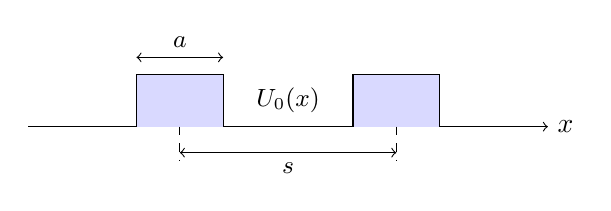
\begin{tikzpicture}[scale=0.55]
\draw[->] (-6,0) -- (6,0) node[right] {$x$};
\fill[blue!15] (-3.5,0) rectangle (-1.5,1.2); \draw (-3.5,0) -- (-3.5,1.2) -- (-1.5,1.2) -- (-1.5,0);
\fill[blue!15] (1.5,0) rectangle (3.5,1.2); \draw (1.5,0) -- (1.5,1.2) -- (3.5,1.2) -- (3.5,0);
\draw[<->] (-3.5,1.6) -- (-1.5,1.6) node[midway,above] {\small $a$};
\draw[<->] (-2.5,-0.6) -- (2.5,-0.6) node[midway,below] {\small $s$};
\draw[dashed] (-2.5,0) -- (-2.5,-0.8); \draw[dashed] (2.5,0) -- (2.5,-0.8);
\node at (0,0.6) {\small $U_0(x)$};
\end{tikzpicture}
\end{center}
\begin{enumerate}
\item Determine la forma funcional de la directividad normalizada en campo lejano $H_N(\theta)$. \pts{1.0 punto}
\item Determine el ancho cero a cero del lóbulo principal (en grados). \pts{0.5 puntos}
\item Determine el ancho a $-3$ dB (en grados). Use la tabla de $\mathrm{sinc}(x)$ que se da abajo. \pts{1.0 punto}
\item ¿A cuántos dB por debajo del pico del lóbulo principal está la presión radiada a $15^\circ$? ¿Hay lóbulos secundarios casi tan altos como el principal? Explique por qué. \pts{0.5 puntos}
\end{enumerate}
\begin{center}\small
\begin{tabular}{c|c||c|c||c|c||c|c}
$x$ & sinc$(x)$ & $x$ & sinc$(x)$ & $x$ & sinc$(x)$ & $x$ & sinc$(x)$\\\hline
0.02 & 0.999 & 0.18 & 0.948 & 0.34 & 0.820 & 0.50 & 0.637\\
0.04 & 0.997 & 0.20 & 0.935 & 0.36 & 0.800 & 0.52 & 0.611\\
0.06 & 0.994 & 0.22 & 0.922 & 0.38 & 0.779 & 0.54 & 0.585\\
0.08 & 0.990 & 0.24 & 0.908 & 0.40 & 0.757 & 0.56 & 0.558\\
0.10 & 0.984 & 0.26 & 0.892 & 0.42 & 0.734 & 0.58 & 0.532\\
0.12 & 0.976 & 0.28 & 0.876 & 0.44 & 0.711 & 0.60 & 0.505\\
0.14 & 0.968 & 0.30 & 0.858 & 0.46 & 0.687 & & \\
0.16 & 0.958 & 0.32 & 0.840 & 0.48 & 0.662 & &
\end{tabular}
\end{center}

\question{Pregunta 4: La ecuación de onda}{3.0 puntos}
Una fuente puntual en aire ($c = 343$ m/s, $\rho_0 = 1.21$ kg/m$^3$) radia a 1 kHz un campo de presión con simetría radial dado por
\begin{equation}
p(r,t) = \frac{A}{r}\,e^{j(\omega t - kr)}
\end{equation}
Recuerde que, con simetría radial, $\nabla^2 p = \dfrac{1}{r}\dfrac{\partial^2 (r p)}{\partial r^2}$.
\begin{enumerate}
\item Demuestre que este campo satisface la ecuación de onda. \pts{1.0 punto}
\item Dé expresiones explícitas y simplificadas de la velocidad de partícula, el desplazamiento de partícula y la impedancia acústica específica. \pts{1.0 punto}
\item ¿A partir de qué distancia el módulo de la impedancia acústica específica difiere en menos de 10\% de la impedancia característica? ¿Y a partir de qué distancia el desfase entre presión y velocidad de partícula es menor que $10^\circ$? \pts{0.5 puntos}
\item A 1 m se mide un nivel de presión sonora de 80 dB SPL. Calcule la intensidad, la potencia acústica de la fuente y el nivel a 4 m. \pts{0.5 puntos}
\end{enumerate}

\sect{Rayos X}

\question{Pregunta 5: Radiografía de proyección con dos energías}{3.0 puntos}
Un antebrazo se modela como una capa de hueso de espesor desconocido $x_b$ y una capa de músculo de espesor desconocido $x_m$, atravesadas por el mismo rayo. Dos mediciones monoenergéticas dan $I/I_0 = 1.74\times10^{-2}$ a 30 keV e $I/I_0 = 0.187$ a 60 keV. Use los coeficientes de atenuación lineal: hueso $1.5$ cm$^{-1}$ (30 keV) y $0.45$ cm$^{-1}$ (60 keV); músculo $0.36$ cm$^{-1}$ (30 keV) y $0.20$ cm$^{-1}$ (60 keV).
\begin{enumerate}
\item Determine $x_b$ y $x_m$. \pts{2.0 puntos}
\item Calcule el contraste hueso/músculo $C = 1 - e^{-(\mu_b-\mu_m)x_b}$ a cada energía. ¿Con qué energía hay más contraste y por qué? ¿Cuál es el costo? \pts{1.0 punto}
\end{enumerate}

\sect{Tomografía computarizada}

\question{Pregunta 6: Proyecciones y retroproyección}{2.0 puntos}
Un objeto está formado por un cuadrado de 2 cm de lado ($\mu = 0.2$ cm$^{-1}$) centrado en el origen, que contiene en su centro un inserto circular de radio 0.5 cm ($\mu = 0.5$ cm$^{-1}$).
\begin{center}
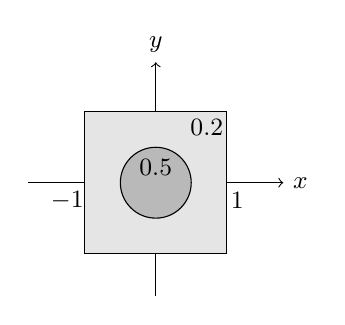
\begin{tikzpicture}[scale=0.9]
\draw[->] (-1.8,0) -- (1.8,0) node[right] {\small $x$};
\draw[->] (0,-1.6) -- (0,1.7) node[above] {\small $y$};
\fill[gray!20] (-1,-1) rectangle (1,1); \draw (-1,-1) rectangle (1,1);
\fill[gray!55] (0,0) circle (0.5); \draw (0,0) circle (0.5);
\node[font=\small] at (0.72,0.78) {0.2}; \node[font=\small] at (0,0.22) {0.5};
\node[font=\small] at (1.15,-0.25) {1}; \node[font=\small] at (-1.25,-0.25) {$-1$};
\end{tikzpicture}
\end{center}
\begin{enumerate}
\item Obtenga la proyección $g(p,\theta)$ a $\theta = 0^\circ$ para todo $p$ y dibújela indicando los valores en $p = 0$, $\pm0.5$ y $\pm1$ cm. \pts{1.0 punto}
\item Calcule $g(0, 45^\circ)$. \pts{0.5 puntos}
\item Usando solo las proyecciones a $0^\circ$ y $90^\circ$, calcule el valor retroproyectado (sin filtro) en el origen. ¿Por qué la retroproyección sin filtro produce una imagen borrosa? \pts{0.5 puntos}
\end{enumerate}

\end{document}
